%!TEX root = MS42.tex
\section{Software Environment}
\subsection{Robot Software Development}
The middleware software used to implement the robot software is \textit{Robot Operating System} (mostly known as ROS) \cite{webros}. Actually, ROS is not just an operating system, it's a complete ecosystem providing libraries, hardware abstraction, device drivers, visualizers, message-passing and package management. 

	% \subsubsection{How ROS Works}
	% Basically, the ROS system is based on nodes, topics, messages and services, allowing the developer to work on a simple and modular code structure.

	% \subparagraph*{Nodes}
	% \textit{Nodes} are processes that perform a specific task. They can use \textit{topics} to communicate between each other and use \textit{services} to handle external operations, e.g.\ a remote procedure call.

	% \subparagraph*{Topics}
	% \textit{Topics} are the transport system used to delivery \textit{messages} between \textit{nodes}. They are based on the \textit{publish/subscribe} semantics, so that a node sends out a message by publishing it on a specific topic. On the other hand, a node will subscribe to the appropriate topic to which it is interested.

	% \subparagraph*{Messages}
	% \textit{Messages} are simply structures of data of typed fields. Just like \textit{C}, they support both standard and user-defined types, as well as nested and complex structures.

	% \subparagraph*{Services}
	% The \textit{publish/subscribe} model, even being a flexible and strong communication system, can't afford the \textit{request/reply} interactions, which is managed by the \textit{services}. An example of usage could be a situation in which a node has executed a task and needs a feedback or an acknowledge for it.

\subsection{Simulation Environment}
During the process of building robot applications, it's clearly not convenient to perform code debug and tests on the real robot. Therefore, the developer needs a simulated environment in which the behaviour of the real robot can be emulated via software in an as precise as possible way, replicating model dynamics, joints and links properties, loads handling and so on. The simulation software used for this purpose is \textit{Gazebo} \cite{webgazebo}, which offers a strict interaction with ROS, providing a realistic rendering of the robot along with its real time ROS-controlled behavior. 

\begin{figure}[H]
\centering
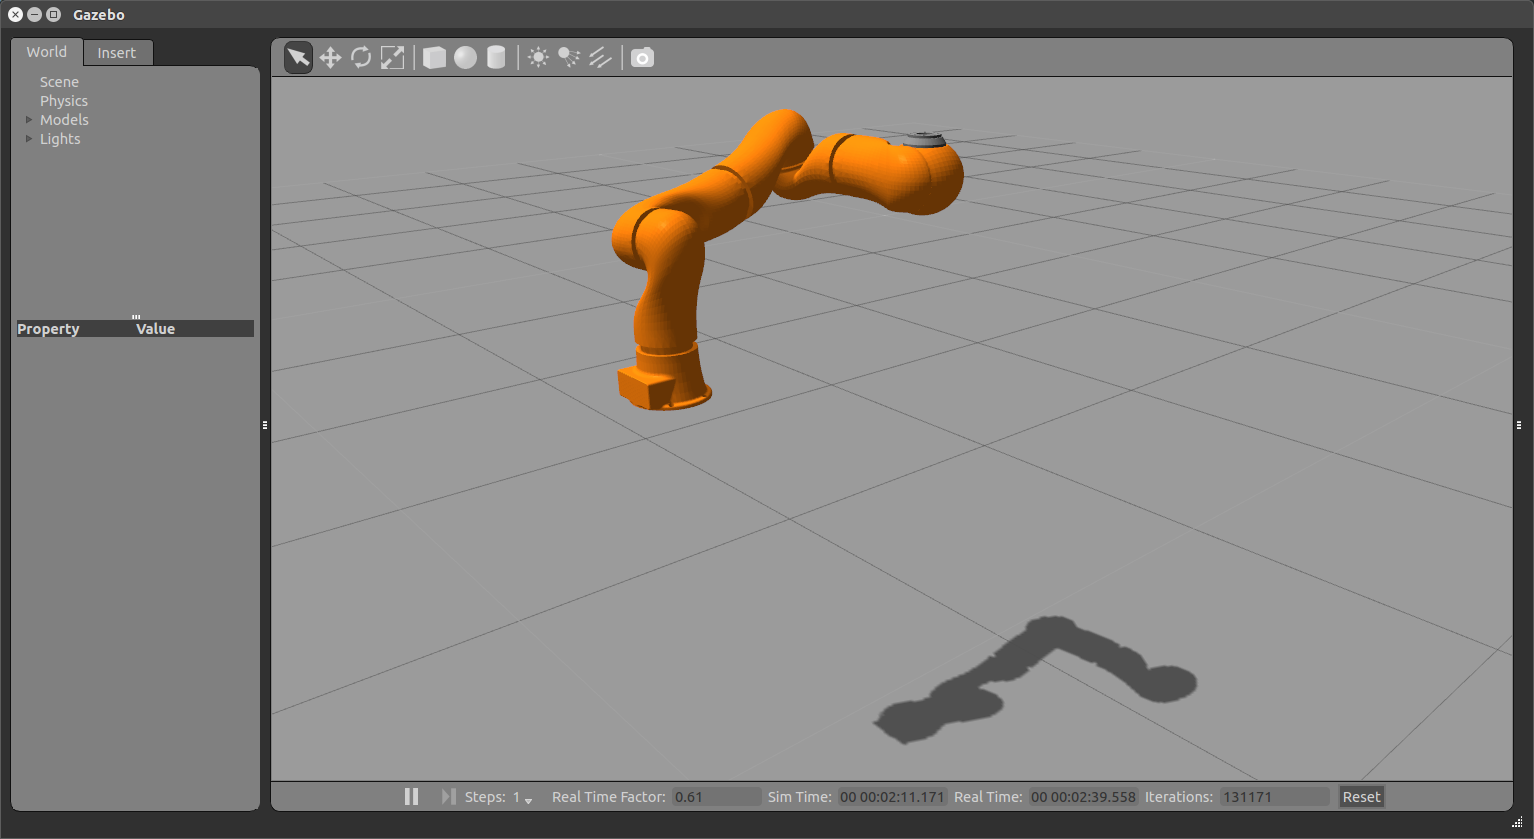
\includegraphics[width=\textwidth]{gazebo} 
\caption{Gazebo Simulator with KUKA LWR IV robot}
\end{figure}


\subsubsection{How Gazebo Works}
To render the robot, the developer has to build a XML file describing all elements of the robot following a tree structure. This file is easily built using the robot focused DSL (\textit{Domain Specific Language}) named URDF (\textit{Unified Robot Description Format}). Gazebo has the task of parsing the URDF model and, through a publish/subscribe system with the ROS nodes and topics, it can apply the user-defined algorithms and control laws to the simulated robot.

\subsection{Additional Tools}
\subsubsection{RViz}
Another software to mention, used mainly in simulation but also during real experiments, is \textit{RViz}, which is a 3D visualization tool included in ROS. It has been useful not only to monitor the current robot configuration (joint states, pose, orientation) but it's also capable of plotting executed trajectories.

\subsubsection{Kinematics and Dynamics Library (KDL)}
A great and valid support in coding has been given by the \textit{Kinematics and Dynamics Library} (KDL), a software framework providing class libraries for robot modeling, as well as computation of forward and inverse chain kinematics and dynamics, motion specification and so on \cite{webkdl}.

\begin{figure}[H]
\centering
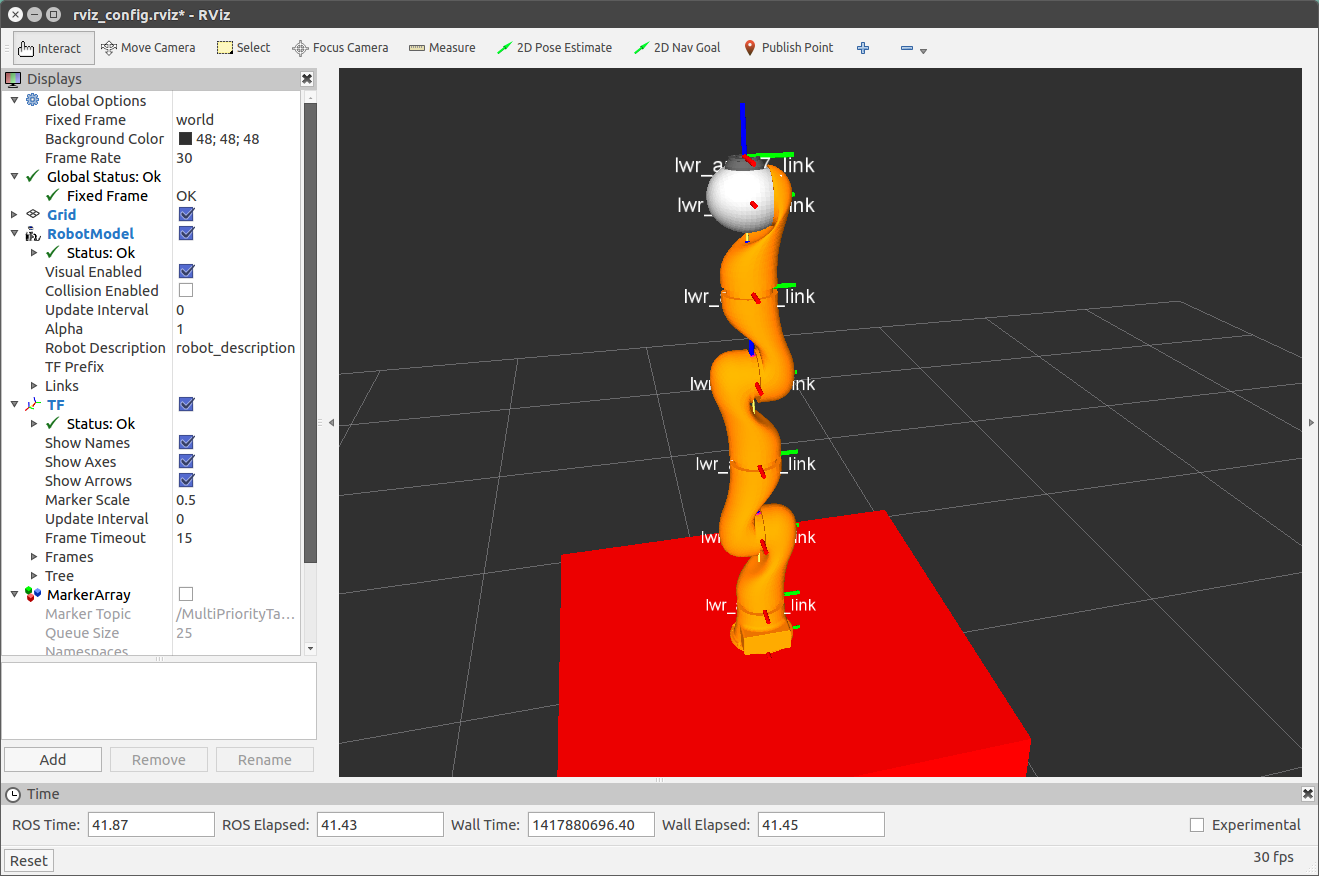
\includegraphics[width=\textwidth]{rviz} 
\caption{Visualization of the KUKA LWR IV robot in RViz}
\end{figure}


\newpage